\documentclass[14pt]{extbook}
\usepackage{multicol, enumerate, enumitem, hyperref, color, soul, setspace, parskip, fancyhdr} %General Packages
\usepackage{amssymb, amsthm, amsmath, bbm, latexsym, units, mathtools} %Math Packages
\everymath{\displaystyle} %All math in Display Style
% Packages with additional options
\usepackage[headsep=0.5cm,headheight=12pt, left=1 in,right= 1 in,top= 1 in,bottom= 1 in]{geometry}
\usepackage[usenames,dvipsnames]{xcolor}
\usepackage{dashrule}  % Package to use the command below to create lines between items
\newcommand{\litem}[1]{\item#1\hspace*{-1cm}\rule{\textwidth}{0.4pt}}
\pagestyle{fancy}
\lhead{Progress Quiz 3}
\chead{}
\rhead{Version A}
\lfoot{3148-2249}
\cfoot{}
\rfoot{Spring 2021}
\begin{document}

\begin{enumerate}
\litem{
Write the equation of the line in the graph below in Standard form $Ax+By=C$. Then, choose the intervals that contain $A, B, \text{ and } C$.
\begin{center}
    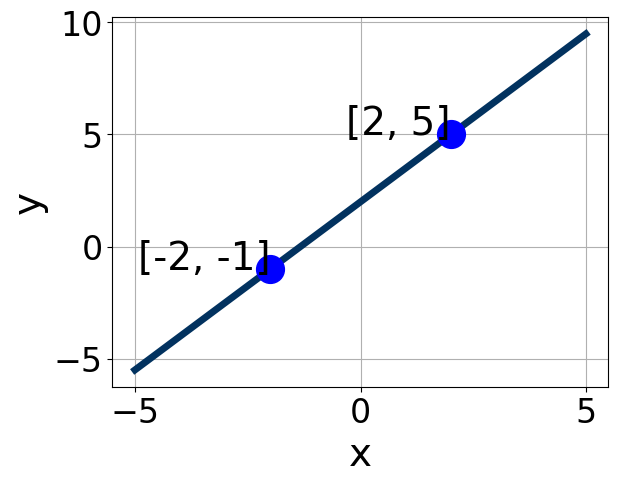
\includegraphics[width=0.5\textwidth]{../Figures/linearGraphToStandardCopyA.png}
\end{center}
\begin{enumerate}[label=\Alph*.]
\item \( A \in [0.2, 1.2], \hspace{3mm} B \in [-4.6, 0.3], \text{ and } \hspace{3mm} C \in [1, 6] \)
\item \( A \in [1.5, 4.1], \hspace{3mm} B \in [3.3, 6.4], \text{ and } \hspace{3mm} C \in [-26, -22] \)
\item \( A \in [1.5, 4.1], \hspace{3mm} B \in [-5.6, -3.3], \text{ and } \hspace{3mm} C \in [23, 30] \)
\item \( A \in [-5.1, 0.1], \hspace{3mm} B \in [-5.6, -3.3], \text{ and } \hspace{3mm} C \in [23, 30] \)
\item \( A \in [0.2, 1.2], \hspace{3mm} B \in [0.6, 3.9], \text{ and } \hspace{3mm} C \in [-8, -1] \)

\end{enumerate} }
\litem{
Solve the equation below. Then, choose the interval that contains the solution.\[ -2(8x + 10) = -15(-16x + 19) \]\begin{enumerate}[label=\Alph*.]
\item \( x \in [0.84, 1.11] \)
\item \( x \in [1.17, 1.23] \)
\item \( x \in [1.24, 1.47] \)
\item \( x \in [-1.22, -1.11] \)
\item \( \text{There are no real solutions.} \)

\end{enumerate} }
\litem{
Solve the equation below. Then, choose the interval that contains the solution.\[ -4(-15x + 16) = -3(5x + 13) \]\begin{enumerate}[label=\Alph*.]
\item \( x \in [1.35, 1.79] \)
\item \( x \in [1.88, 2.83] \)
\item \( x \in [-2.09, -0.66] \)
\item \( x \in [-0.63, 0.39] \)
\item \( \text{There are no real solutions.} \)

\end{enumerate} }
\litem{
Find the equation of the line described below. Write the linear equation as $ y=mx+b $ and choose the intervals that contain $m$ and $b$.\[ \text{Parallel to } 4 x - 7 y = 13 \text{ and passing through the point } (-9, -3). \]\begin{enumerate}[label=\Alph*.]
\item \( m \in [0.79, 2.64] \hspace*{3mm} b \in [1.4, 3.2] \)
\item \( m \in [-0.03, 1.18] \hspace*{3mm} b \in [4.8, 6.4] \)
\item \( m \in [-0.03, 1.18] \hspace*{3mm} b \in [-4.2, -1.9] \)
\item \( m \in [-0.72, 0.26] \hspace*{3mm} b \in [-11.3, -6.9] \)
\item \( m \in [-0.03, 1.18] \hspace*{3mm} b \in [1.4, 3.2] \)

\end{enumerate} }
\litem{
Find the equation of the line described below. Write the linear equation as $ y=mx+b $ and choose the intervals that contain $m$ and $b$.\[ \text{Perpendicular to } 7 x - 8 y = 8 \text{ and passing through the point } (-9, 7). \]\begin{enumerate}[label=\Alph*.]
\item \( m \in [-1.52, -1.14] \hspace*{3mm} b \in [-4.2, -2.4] \)
\item \( m \in [0.78, 1.51] \hspace*{3mm} b \in [17.1, 17.9] \)
\item \( m \in [-1.52, -1.14] \hspace*{3mm} b \in [14.3, 17] \)
\item \( m \in [-1.52, -1.14] \hspace*{3mm} b \in [3.1, 4.1] \)
\item \( m \in [-1.03, -0.86] \hspace*{3mm} b \in [-4.2, -2.4] \)

\end{enumerate} }
\litem{
First, find the equation of the line containing the two points below. Then, write the equation as $ y=mx+b $ and choose the intervals that contain $m$ and $b$.\[ (10, -2) \text{ and } (-10, 5) \]\begin{enumerate}[label=\Alph*.]
\item \( m \in [-1.26, 0.18] \hspace*{3mm} b \in [12, 21] \)
\item \( m \in [0.34, 1.09] \hspace*{3mm} b \in [5.5, 9.5] \)
\item \( m \in [-1.26, 0.18] \hspace*{3mm} b \in [-16, -7] \)
\item \( m \in [-1.26, 0.18] \hspace*{3mm} b \in [-2.5, -0.5] \)
\item \( m \in [-1.26, 0.18] \hspace*{3mm} b \in [-0.5, 3.5] \)

\end{enumerate} }
\litem{
Write the equation of the line in the graph below in Standard form $Ax+By=C$. Then, choose the intervals that contain $A, B, \text{ and } C$.
\begin{center}
    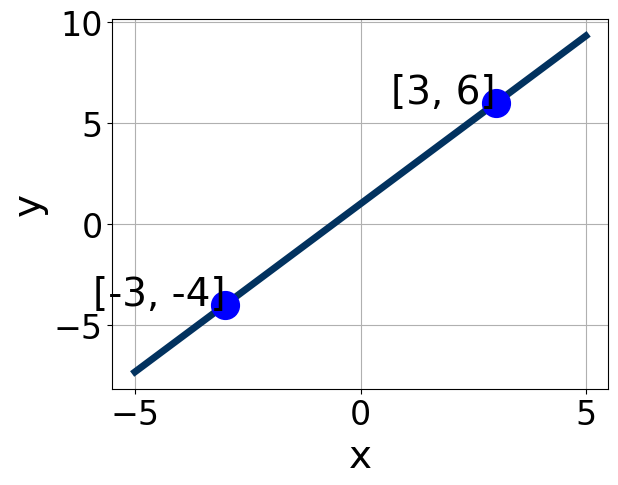
\includegraphics[width=0.5\textwidth]{../Figures/linearGraphToStandardA.png}
\end{center}
\begin{enumerate}[label=\Alph*.]
\item \( A \in [4, 11], \hspace{3mm} B \in [2.04, 4.5], \text{ and } \hspace{3mm} C \in [2.44, 3.39] \)
\item \( A \in [4, 11], \hspace{3mm} B \in [-3.74, -2.11], \text{ and } \hspace{3mm} C \in [-5.31, -1.46] \)
\item \( A \in [-4.67, 1.33], \hspace{3mm} B \in [0.56, 1.52], \text{ and } \hspace{3mm} C \in [0.6, 1.24] \)
\item \( A \in [-6, -2], \hspace{3mm} B \in [2.04, 4.5], \text{ and } \hspace{3mm} C \in [2.44, 3.39] \)
\item \( A \in [-4.67, 1.33], \hspace{3mm} B \in [-1.1, -0.48], \text{ and } \hspace{3mm} C \in [-1.62, -0.58] \)

\end{enumerate} }
\litem{
Solve the linear equation below. Then, choose the interval that contains the solution.\[ \frac{6x + 7}{7} - \frac{4x -6}{5} = \frac{7x + 7}{8} \]\begin{enumerate}[label=\Alph*.]
\item \( x \in [1.18, 2.06] \)
\item \( x \in [6.93, 7.83] \)
\item \( x \in [-1.33, -0.38] \)
\item \( x \in [-1.31, 0.5] \)
\item \( \text{There are no real solutions.} \)

\end{enumerate} }
\litem{
Solve the linear equation below. Then, choose the interval that contains the solution.\[ \frac{-4x + 4}{7} - \frac{-5x -3}{2} = \frac{7x -9}{6} \]\begin{enumerate}[label=\Alph*.]
\item \( x \in [-1, 0.5] \)
\item \( x \in [-23.4, -20.9] \)
\item \( x \in [-5.9, -3.7] \)
\item \( x \in [-0.6, 2.8] \)
\item \( \text{There are no real solutions.} \)

\end{enumerate} }
\litem{
First, find the equation of the line containing the two points below. Then, write the equation as $ y=mx+b $ and choose the intervals that contain $m$ and $b$.\[ (10, -7) \text{ and } (11, 9) \]\begin{enumerate}[label=\Alph*.]
\item \( m \in [-17, -11] \hspace*{3mm} b \in [185, 190] \)
\item \( m \in [16, 22] \hspace*{3mm} b \in [162, 169] \)
\item \( m \in [16, 22] \hspace*{3mm} b \in [-172, -159] \)
\item \( m \in [16, 22] \hspace*{3mm} b \in [-20, -10] \)
\item \( m \in [16, 22] \hspace*{3mm} b \in [-4, 1] \)

\end{enumerate} }
\end{enumerate}

\end{document}